\documentclass[11pt,a4paper]{article}
\usepackage[left=2cm,right=2cm,top=2cm,bottom=3cm]{geometry}
\usepackage{amsmath,amsfonts,amsthm,amssymb,varioref,times, commath}
\usepackage{gensymb}
\usepackage{tikz}
\usepackage{textcomp}
\usepackage{hyperref}
\hypersetup{
 colorlinks=true,
 linkcolor=blue,
 filecolor=magenta, 
urlcolor=cyan,
}
\usepackage{lipsum}
\usepackage{epigraph}
%to resume numbering in a list
\usepackage{enumitem}
%----- arrows 
\usepackage{extarrows}

%    differential equatiosn 
\usepackage{diffcoeff}   %\diff[2]{x}{y}


%%%%%%pour ecrire en français avec les accents
\usepackage[utf8]{inputenc}
\usepackage[T1]{fontenc}
\usepackage{lmodern} % load a font with all the characters
\usepackage{units}
%%%%%%%Image-related packages
\usepackage{wrapfig}
\usepackage{float, graphicx}
\graphicspath{ {./img/} }
\usepackage{subcaption}
\usepackage[export]{adjustbox}

%%%%%%%pour faire des cadres
\usepackage{xcolor}
\usepackage{tcolorbox}
\usepackage{framed}
\usepackage{mdframed}


%%%%%%%chemistry frmulae
\usepackage{chemfig}
\usepackage{chemformula}
\usepackage[version=4]{mhchem}

% -------------- Circuits -------------------
\usepackage[european, straightvoltages]{circuitikz}

% Title & headers
\usepackage[explicit]{titlesec}
% Raised Rule Command:
% Arg 1 (Optional) - How high to raise the rule
% Arg 2 - Thickness of the rule
\newcommand{\raisedrulefill}[2][0ex]{\leaders\hbox{\rule[#1]{1pt}{#2}}\hfill}
\titleformat{\section}{\Large\bfseries}{\thesection. }{0em}{#1\,\raisedrulefill[0.4ex]{1pt}}

% pour ecrire sur +sieurs colonnes
\usepackage{multicol}
\setlength{\columnseprule}{0pt}
\setlength{\columnsep}{60pt}
% Fusion de lignes de tableaux.
\usepackage{multirow}
% Position verticale des lettres dans la ligne de tableau.
\usepackage{array}

% physics -----------------------------------------------------------
\newcommand{\To}{\longrightarrow}
\newcommand{\gpl}{\; g\cdot L^{-1}}
\newcommand{\gpmol}{\; g\cdot mol^{-1}}
\newcommand{\mpl}{\; mol\cdot L^{-1}}
\newcommand{\mps}{\; m\cdot s^{-1}}
\newcommand{\rps}{\; rad\cdot s^{-1}}
\newcommand{\kph}{\; km\cdot h^{-1}}
\newcommand{\mpss}{\; m\cdot s^{-2}}
\newcommand{\Dt}{\Delta t}
\newcommand{\vv}{\vec{v}}
\newcommand{\va}{\vec{a}}
\newcommand{\vp}{\vec{p}}
\newcommand{\vf}{\vec{F}}
\newcommand*{\Vf}[1]{\overrightarrow{F_\ensuremath{{#1}}}}
\newcommand{\es}[1]{\cdot10^{#1}}
\newcommand{\eng}[1]{\textcolor{purple}{(= #1})}
\usepackage{harpoon}
%\newcommand*{\vect}[1]{\overrightharp{\ensuremath{#1}}}
\newcommand*{\Vect}[1]{\overrightarrow{\ensuremath{#1}}}
\newcommand{\pfd}[1]{\sum \vec{F}_{ext_{#1}} &= \od{\vp_{#1}}{t} = m\cdot\va_{#1}}
\newcommand{\C}{\degree C}
\newcommand{\Delt}{\Delta t}

% --- Circuits ------------
\newcommand{\bipole}[1]{
\begin{circuitikz} \draw
(0,0) to[ #1 ] (2,0); 
\end{circuitikz} {\hspace{5mm}}}

% Chimie ---------------------------------
\newcommand{\oxo}{\ce{H3O+}_{(aq)}}
\newcommand{\eau}{\ce{H2O}_{(\ell)}}
\newcommand{\OH}{\ce{HO-}_{(aq)}}
\newcommand{\AH}{\ce{AH}_{(aq)}}
\newcommand{\A}{\ce{A-}_{(aq)}}
\newcommand{\MnO}{\ce{MnO_4^{-}}}
\newcommand{\conc}[1]{\left[{#1}\right]}
\newcommand{\couple}[2]{\ce{#1/#2}}


% Environnements ------------------------
\newcounter{exo}
\newenvironment{exo}[1][]
{\refstepcounter{exo} \begin{shaded}\noindent $\triangleright \quad$\textbf{Exercice~\theexo. #1} } { \end{shaded}}
\newenvironment{eg}
{\begin{shaded} \textbf{Exemple:} } { \end{shaded}}

\newenvironment{defn}[1]
{\begin{leftbar}\noindent \textbf{Définition :\textit{ \quad #1}} } { \end{leftbar}}

%\newenvironment{rmrq}
%{\begin{shaded} \textbf{Remarque.\quad } \itshape } { \end{shaded}}
\newenvironment{rmrq}
{\begin{mdframed}[backgroundcolor=blue!10, linewidth=0pt] \textbf{Remarque.\quad } \itshape } { \end{mdframed}}

\newenvironment{python}
{\begin{shaded} \textbf{A faire en PYTHON}\\ \itshape } { \end{shaded}}

% Shading colour -----------------------------
\definecolor{shadecolor}{gray}{0.9}

\date{}
\author{}

\renewcommand*\contentsname{Résumé}









% Title & headers 
\usepackage{fancyhdr}
\pagestyle{fancy}
\fancyhf{}
\lhead{SciPhy : Terminale spé}
\rhead{$\chi $ - 3b : Réactions acide/base}
\chead{2020-28}
\rfoot{Page \thepage}
\lfoot{\textcopyright\; S Zayyani}
\renewcommand{\footrulewidth}{0.1pt}% default is 0pt

\title{\large Chimie - Chapitre 3b \\ \LARGE  Les réactions acidobasiques}



\setlength{\parindent}{0mm}
\setlength{\parskip}{2mm}

\setlength{\intextsep}{6pt}%
\setlength{\columnsep}{5pt}%

\begin{document}
\maketitle
\vspace{-1cm}
\begin{tcolorbox}[title=Notions de la classe de première à rappeler]
calcul d'un logarithme ; solvatation d'un proton libre dans l'eau ; Concentration molaire
%\tcblower
\end{tcolorbox}
\tableofcontents

\section{La constante d'acidité} % --------------- SECTION------------
Comme toutes réactions chimiques, les réactions acido-basiques se trouvent souvent en équilibre chimique, et peuvent donc être caractérisées par une constante d’équilibre, notée $K_a$. 


% \begin{wraptable}{l}{0.35\textwidth}
% \begin{tabular}{c||c}
% Couple acide/base & pK_a \\ \hline
% \oxo/\eau & 0,00 \\ 
% \ce{HF}_{(aq)}/\ce{F-}_{(aq)} & 3,20 \\ 
% \ce{HCOOH}_{(aq)}/\ce{HCOO-}_{(aq)} & 3,75 \\ 
% \ce{CH3COOH}_{(aq)}/\ce{CH3COO-}_{(aq)} & 4,76 \\ 
% \ce{NH4+}_{(aq)}/\ce{NH3}_{(aq)} & 10,3 \\ 
% \ce{HCO3-}_{(aq)}/\ce{CO3^2-}_{(aq)} & 10,3 \\ 
% \eau/\OH & 14,0
% \end{tabular}
% \caption{Quelques couples acide/base et leurs $pK_a$}
% \end{wraptable}
\begingroup
\begin{wrapfigure}{r}{0.3\textwidth}
  \centering
  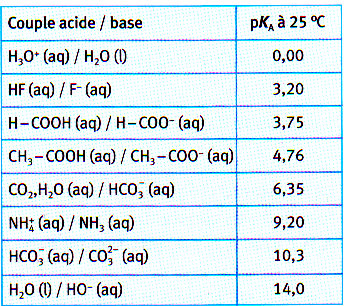
\includegraphics[width=0.95\linewidth]{imgs/c3/ka.jpg}
\end{wrapfigure}

\begin{defn}{Constante d'acidité\eng{acid dissociation constant}}
\begin{itemize}
    \item La constante d’équilibre de la réaction d’un acide $AH$ avec l’eau est notée $K_a$. On l’appelle \textbf{constante d’acidité} du couple $\ce{AH}_{(aq)}/\ce{A-}_{(aq)} $ .  
    \item La réaction de la mise en solution de $AH$ est :
    \[\ce{AH}_{(aq)} + \eau \rightleftharpoons \ce{A-}_{(aq)} + \oxo \]
    avec la constante d'acidité 
    \[ K_a = \dfrac{[\oxo]_{éq}\cdot[ \ce{A-}]_{éq} }{ [\ce{A-}]_{éq} }  \]
    \item À partir de la constante d'acidité nous définissons le $pK_a$, qui caractérise le couple acide/base : 
    \[
    pK_a = -\log(K_a) \Longleftrightarrow K_a = 10^{-pK_a}
    \]
\end{itemize}
\end{defn}

\endgroup

\begin{rmrq}

L'acidité d'une solution aqueuse est en fait due à la présence des ions oxonium $ \oxo $ dans la solution. 

Il est courant, par exemple, qu’on parle tout simplement d’acide sulfurique pour désigner la solution aqueuse.  Or, pour l’acide sulfurique, cette appellation est impropre, car on confond alors l’acide sulfurique, et la solution obtenue en faisant réagir l’acide avec l’eau. 

Plus le $pK_a$ du couple est grand (ou plus la constante $K_a$  est petite) moins l’acide se dissocie dans l’eau. 

Certains acides comme $\ce{HC\ell}$ (acide chlorhydrique), $\ce{HNO3}$ (acide nitrique), $\ce{H2SO4}$  (acide sulfurique) réagissent de manière \textbf{totale}. Ils ont donc une constante $K_a$  très élevée, et un $pK_a$  négatif. Ces acides ne peuvent pas exister sous forme moléculaire dans l’eau. 
\end{rmrq}

\begin{exo}
Pour augmenter le $pH$ d'une piscine, on ajoute du carbonate de sodium $\ce{Na2CO3}_{(g)}$. L'ion carbonate réagit avec l'eau. La constante 
d'acidité du couple $ \ce{HCO3-}_{(aq)}/\ce{CO3^2-}_{(aq)} $ est égale à : $K_a_1 = 5,0\es{-11}$
\begin{enumerate}
    \item L'eau réagit-elle en tant que base ou en tant qu'acide? Quel est le couple de l'eau impliqué? 
    \item Donner les expressions des constantes d'acidités $K_A_1$ du couple $ \ce{HCO3-}_{(aq)}/\ce{CO3^2-}_{(aq)} $ et $K_A_2$ du couple de l'eau impliqué. Quelle est 1a va1eur de $K_a-2$ à $25\degree C$?
    \item Écrire l'équation de la réaction acido-basique qui a lieu. 
    \item Exprimer puis calculer sa constante d'équilibre à $25\degree C$. 
\end{enumerate}
\end{exo}

\section{Force des acides et des bases}% --------------- SECTION------------

\begin{defn}{Acide fort \& faible}
\begin{itemize}
    \item 	On dit qu’un acide est d’autant \textbf{plus fort} que le taux d’avancement final $\tau = \dfrac{x_{éq}}{x_{max}}$ de sa réaction avec l’eau est grand.
    \item Un acide $\ce{AH}$ est dit \textbf{fort} si toutes les entités introduites dans l’eau se dissocient en libérant un ion hydrogène $\ce{H+}$.  La réaction avec l’eau est donc totale : 
    \[ \ce{AH} + \eau \To \ce{A-} + \oxo  \]
    \item Un acide $\ce{AH}$ est dit \textbf{faible} si une partie seulement des entités introduites dans l’eau se dissocient en libérant un ion hydrogène $\ce{H+}$.  La réaction avec l’eau est donc limitée : 
    \[ \ce{AH} + \eau \rightleftharpoons \ce{A-} + \oxo  \]
    \item 	À température et à concentration de soluté apporté égales, un acide $\ce{AH}$ est d’autant plus fort que la valeur du $pK_a$  est faible. 
    \item Pour une concentration molaire $c$ comprise entre $ 10^{-1} \sim 10^{-6} \mpl$, le $pH$ d’une solution d’acide fort est : $pH=-\log(c)$
\end{itemize}
\end{defn}

\begin{figure}[h]
    \centering
    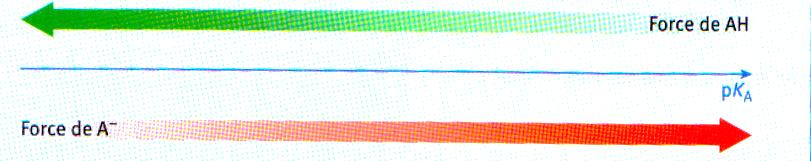
\includegraphics[width=.7\textwidth]{imgs/c3/forceacides.jpg}
\end{figure}

\section{Diagrammes de prédominance}% --------------- SECTION------------

Considérons le couple $\ce{AH}_{(aq)}/\ce{A-}_{(aq)} $. La constante d'acidité s'écrit : 
\begin{align*}
    K_a &= \dfrac{[\oxo]_{éq}\cdot[ \ce{A-}]_{éq} }{ [\ce{AH}]_{éq} }   \\
    &= \dfrac{[\ce{A-}]_{éq} }{ [\ce{AH}]_{éq} }\cdot [\oxo]_{éq} 
\end{align*}
Le $pK_a$ est donc : 

\begin{align*}
    pK_a &= -\log(K_a) \\ 
    &= -\log\Bigg(\dfrac{[\ce{A-}]_{éq} }{ [\ce{AH}]_{éq} }\cdot [\oxo]_{éq} \Bigg) \\
    &= -\log\Bigg(\dfrac{[\ce{A-}]_{éq} }{ [\ce{AH}]_{éq} } \Bigg) - \log\Bigg( [\oxo]_{éq} \Bigg)\\
    &= -\log\Bigg(\dfrac{[\ce{A-}]_{éq} }{ [\ce{AH}]_{éq} } \Bigg) + pH
\end{align*}

Et nous obtenons la relations : 
\[ pH = pK_a +  \log\Bigg(\dfrac{[\ce{A-}]_{éq} }{ [\ce{AH}]_{éq} } \Bigg) \]

que nous pouvons réécrire aussi : 
\[ \dfrac{[\ce{A-}]_{éq} }{ [\ce{AH}]_{éq} }  =  10^{pH - pK_a}\]

À partir de ces deux relations, notamment la dernière nous pouvons déterminer l’\textbf{espèce prédominante} en fonction du $pH$ de la solution (i.e. est-ce que c’est la forme acide ou basique qui présente en majorité). C’est-à-dire :
\begin{itemize}
    \item si $pH = pK_a \Rightarrow \log\Bigg(\dfrac{[\ce{A-}]_{éq} }{ [\ce{AH}]_{éq} } \Bigg)  = 0 $ \textbf{soit} $\dfrac{[\ce{A-}]_{éq} }{ [\ce{AH}]_{éq} } = 1 $
    \item si $pH > pK_a \Rightarrow \log\Bigg(\dfrac{[\ce{A-}]_{éq} }{ [\ce{AH}]_{éq} } \Bigg)  > 0 $ \textbf{soit} $\dfrac{[\ce{A-}]_{éq} }{ [\ce{AH}]_{éq} } > 1 $
    \item si $pH < pK_a \Rightarrow \log\Bigg(\dfrac{[\ce{A-}]_{éq} }{ [\ce{AH}]_{éq} } \Bigg)  < 0 $ \textbf{soit} $\dfrac{[\ce{A-}]_{éq} }{ [\ce{AH}]_{éq} } < 1 $
\end{itemize}

Nous pouvons visualiser ces trois régimes grâce à un diagramme de prédominance

\begin{defn}{Diagramme de prédominance}
\begin{itemize}
    \item Dans un système chimique, on dit qu’une espèce $A$ est prédominante par rapport à une espèce $B$ si $[A]>[B]$
    \begin{itemize}
        \item Si $pH = pK_a \longrightarrow [\ce{A-}]_{éq} =[AH]_éq $ donc il n’y a pas d’espèce prédominante. 
        \item Si $pH > pK_a \longrightarrow [\ce{A-}]_{éq} >[AH]_éq $ donc c'est la forme basique qui prédomine. 
        \item Si $pH < pK_a \longrightarrow [\ce{A-}]_{éq} <[AH]_éq $ donc c'est la forme acide qui prédomine.  
    \end{itemize}
    \item Un diagramme de prédominance représente les zones de $pH$ où les espèces d’un couple acide/base prédominent, comme dans la figure ci-après. 
\end{itemize}
\end{defn}
\begin{figure}[h]
    \centering
    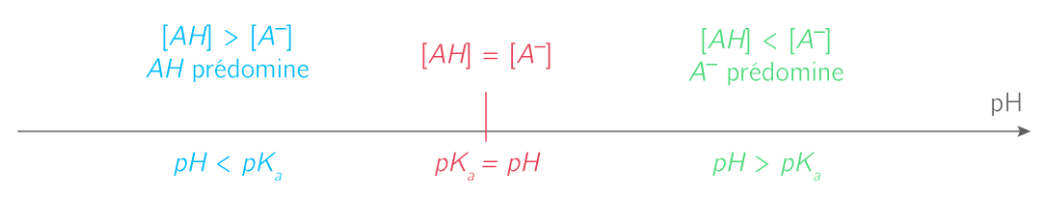
\includegraphics[width=0.9\linewidth]{imgs/c3/predom.png}
    \caption{Diagramme de prédominance pour le couple $\ce{AH}_{(aq)}/\ce{A-}_{(aq)} $}
\end{figure}

\newpage

\section{Titrage $pH$-métrique}% --------------- SECTION------------

Lors d’un titrage pH-métrique, le $pH$ est mesuré après chaque ajout de solution titrante. Contrairement à un titrage avec utilisation d’un indicateur coloré, la solution titrante continue à être versée au-delà de l’équivalence. Nous obtenons de cette manière des $pH$ en ordonnées et des volumes en abscisses, qui nous donnent après avoir été reportés dans un graphique, la courbe du titrage acido-basique (cf. figure ci-après). 
\begin{itemize}
    \item La partie AB où les variations des $pH$ sont assez faibles, avant l’équivalence
    \item La partie BC, appelée « \textbf{la zone de virage} » ou « \textbf{le saut de $pH$} », où se trouve le \textbf{point d’équivalence}
    \item La partie CD où le $pH$ se stabilise, après l’équivalence.
\end{itemize}

\begin{figure}[h]
    \centering
    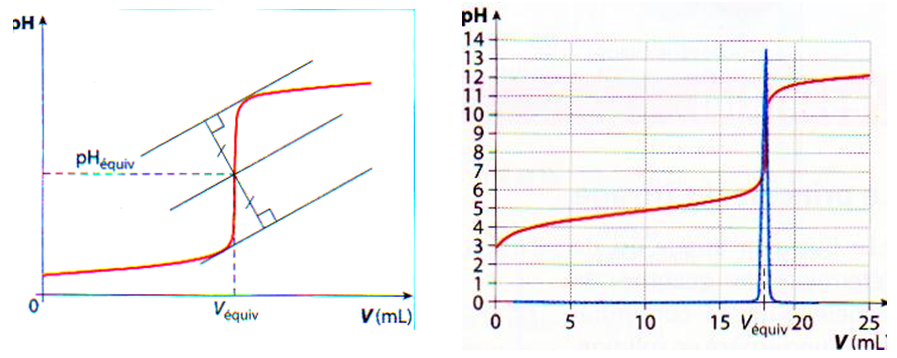
\includegraphics[width=\linewidth]{imgs/c3/titreAB.png}
    \caption{Méthode des tangentes à gauche \& méthode des dérivées à droite}
\end{figure}	 

\begin{figure}[h]
    \centering
    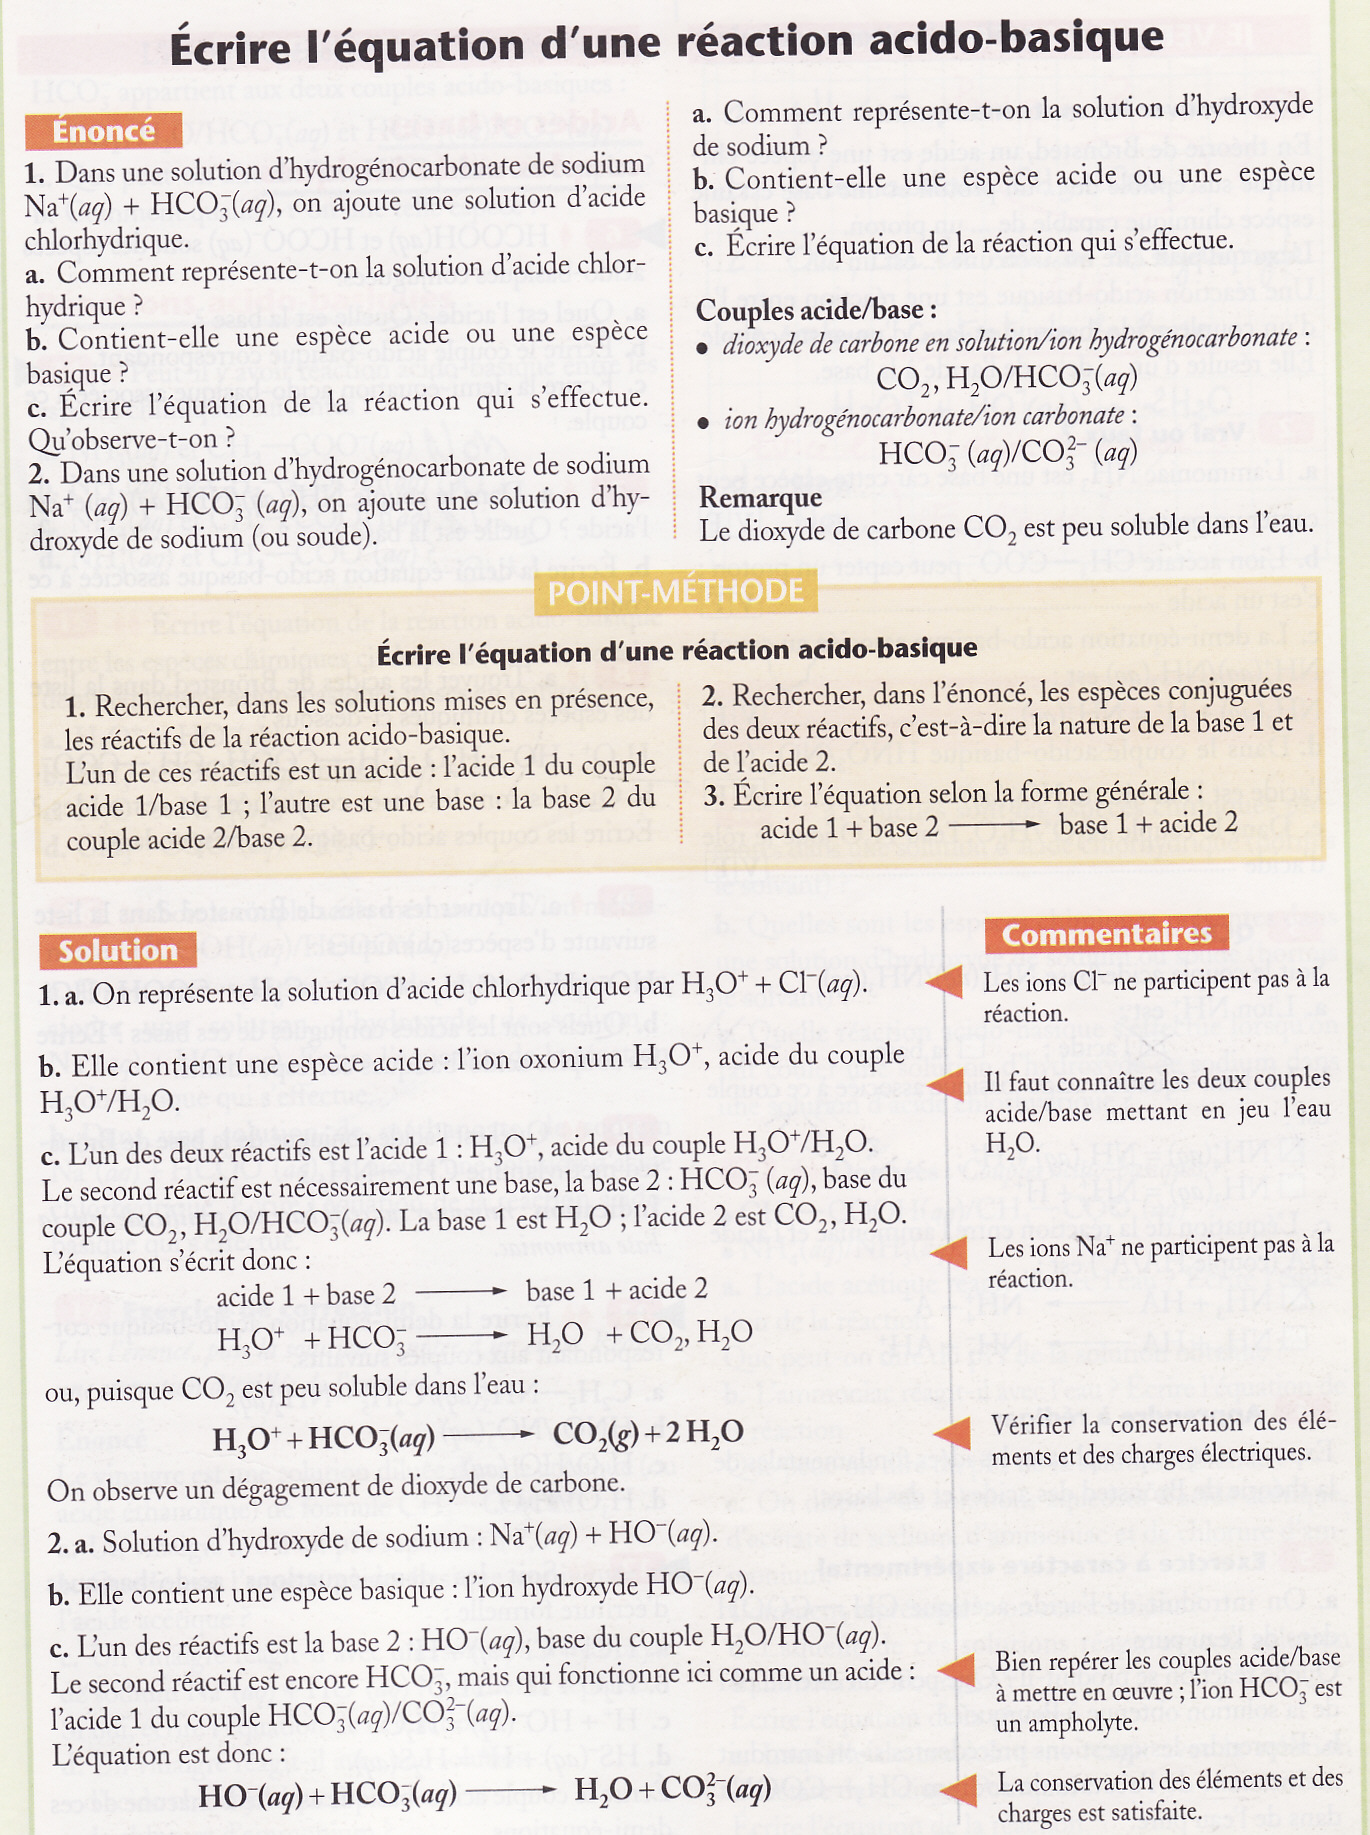
\includegraphics[width=\linewidth]{imgs/c3/xo1.jpg}
\end{figure}

\begin{figure}[h]
    \centering
    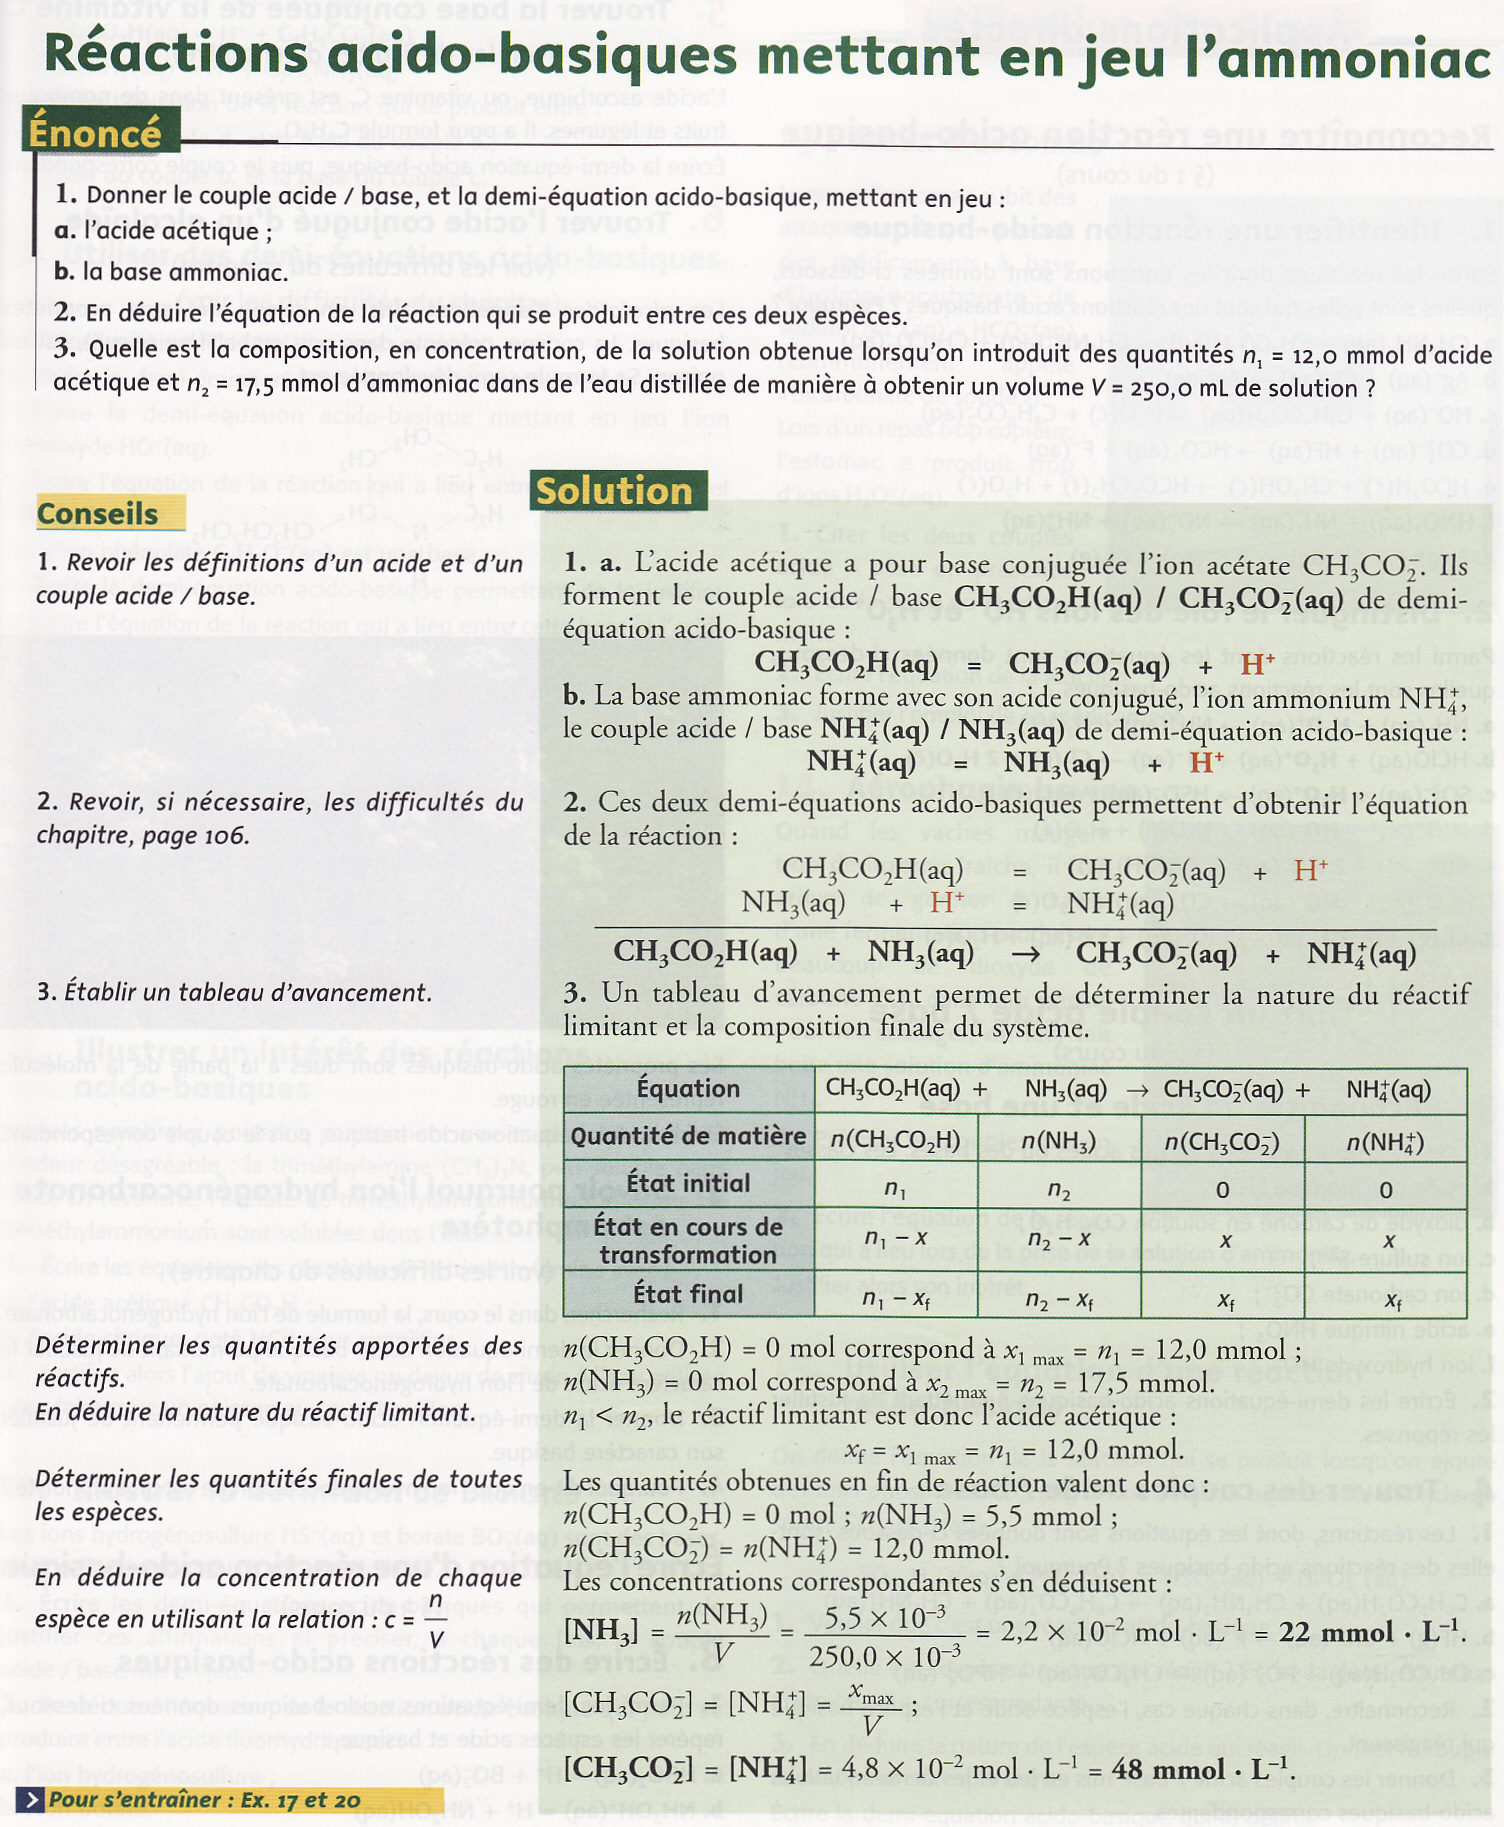
\includegraphics[width=\linewidth]{imgs/c3/xo2.jpg}
\end{figure}
\begin{figure}[h]
    \centering
    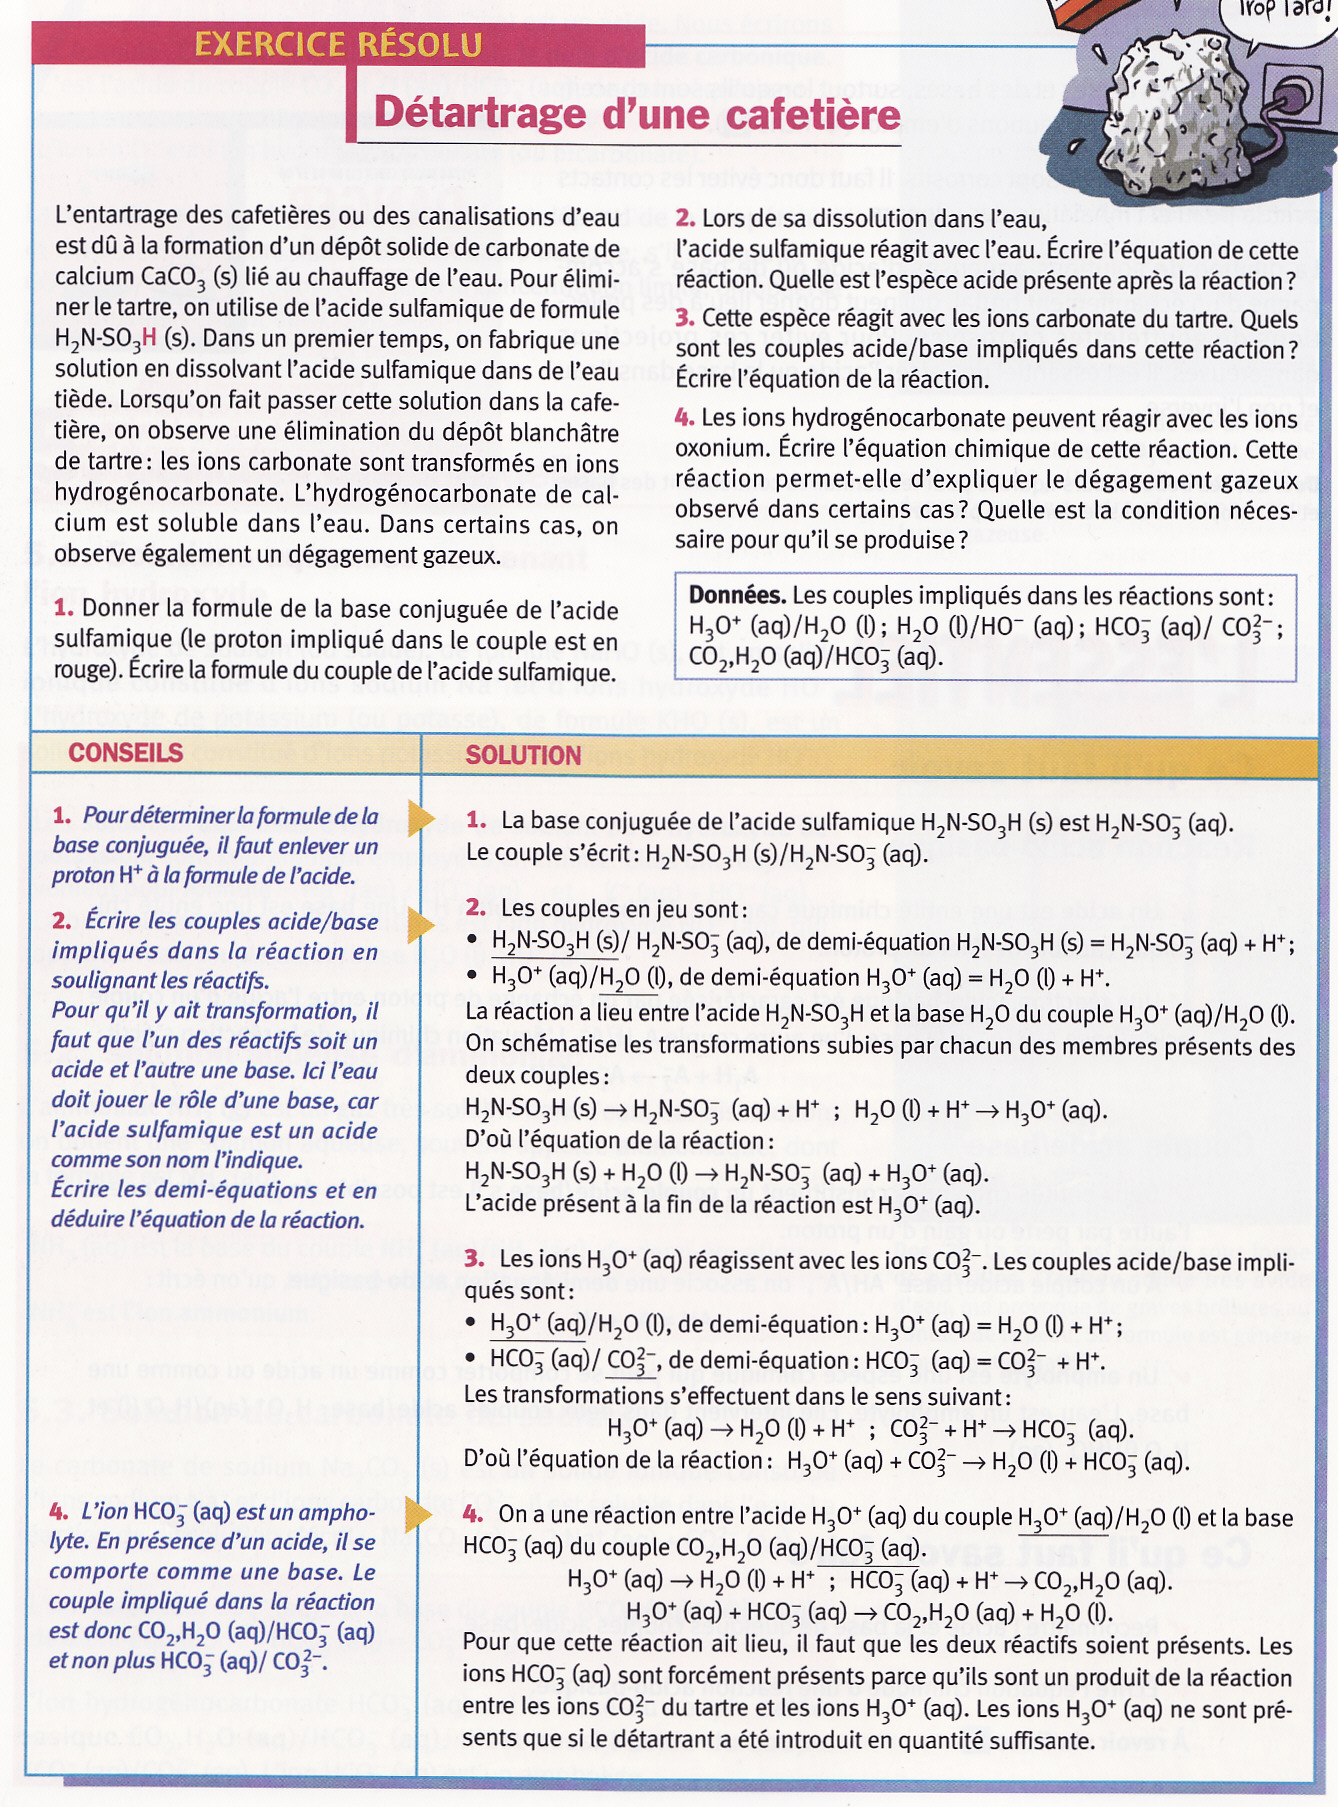
\includegraphics[width=\linewidth]{imgs/c3/xo3.jpg}
\end{figure}
\begin{figure}[h]
    \centering
    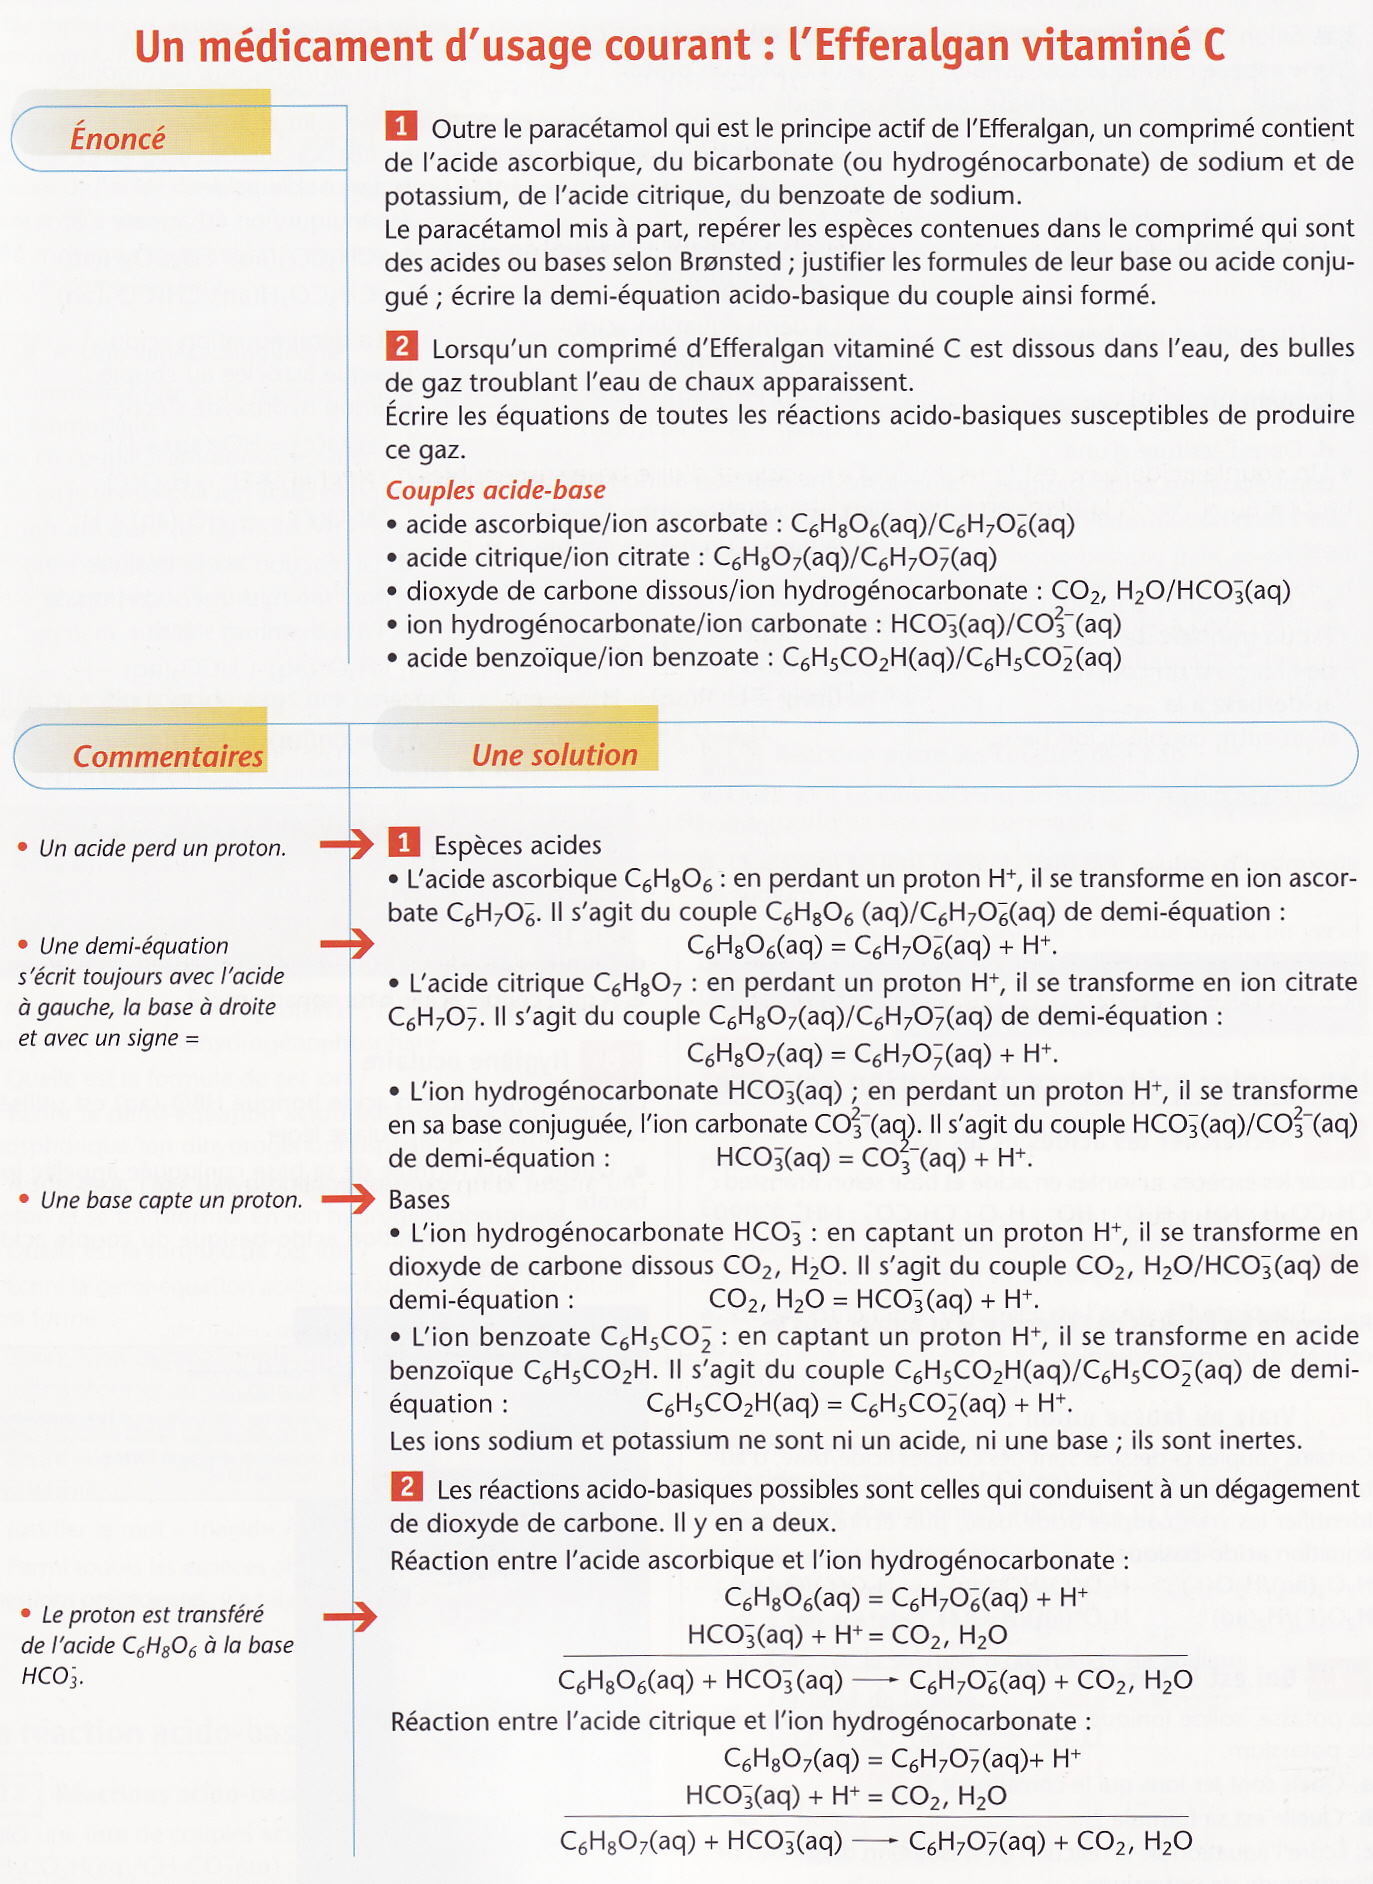
\includegraphics[width=\linewidth]{imgs/c3/xo4.jpg}
\end{figure}

\end{document}

